\subsubsection{\texttt{RF-4}: previsualización del \textit{dashboard}}
\label{subsec:rf4}

La versión de \textit{VSCode4Teaching} tomada como punto de partida para el inicio del presente TFG incluía ya un \textit{dashboard} completamente funcional que requería que el profesor tuviese descargado el ejercicio completo en su propio espacio de trabajo en Visual Studio Code para poder ejecutar las funcionalidades de apertura de ficheros y visualización de diferencias con la plantilla, que se ejecutan mediante botones situados en cada fila de la tabla mostrada en esta visualización.

El presente requisito busca eliminar la necesidad de descargar todos los ficheros de los ejercicios y permitir a los profesores visualizar el \textit{dashboard} ---sin acceso a las funcionalidades anteriormente nombradas--- para el ejercicio que deseen con independencia del que tengan activo en su espacio de trabajo. Este formato de ``previsualización'' conlleva modificaciones del \textit{dashboard}, que únicamente deberá mostrar la columna con las acciones anteriormente citadas si se abre en ``modo completo'' ---es decir, tal como se venía haciendo en versiones anteriores---. Los profesores pueden acceder a la previsualización del \textit{dashboard} de cada ejercicio haciendo uso de un nuevo botón colocado en la barra lateral junto a cada ejercicio, tal como se puede evidenciar en la \referenciaFigura{fig:reqf4-1}. Esta previsualización introduce, además, un elemento gráfico explicativo que aclara al profesor que, en caso de querer ejecutar las acciones de apertura y visualización de diferencias entre archivos, deberá descargar el ejercicio y hacer uso del \textit{dashboard} completo.

\begin{figure}[ht]
    \centering
    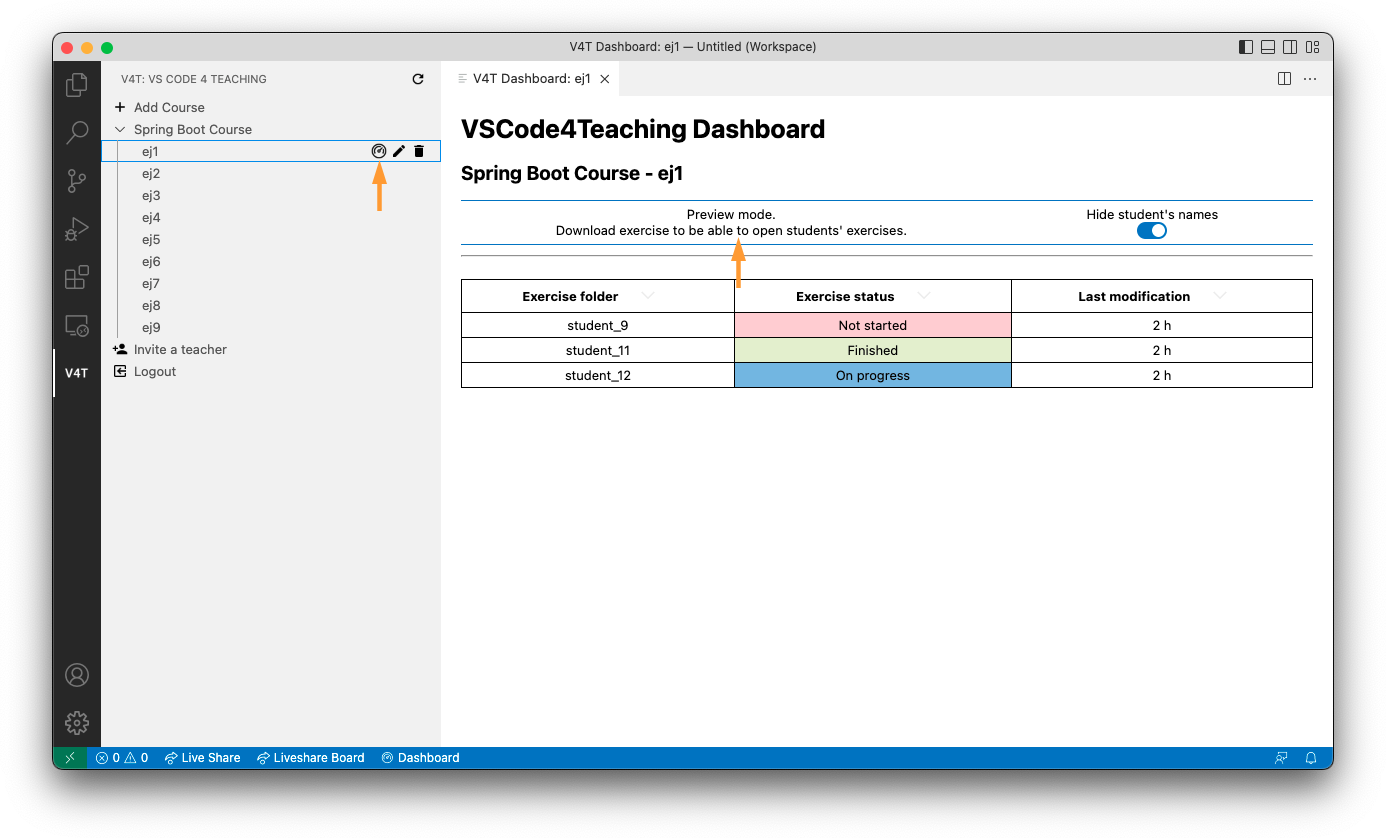
\includegraphics[width=\textwidth]{imagenes/utilizadas/4-3-implementacion/rf4-1.png}
    \caption{Captura de la extensión en la que se muestran los elementos de la GUI que permiten distinguir el modo de previsualización del \textit{dashboard}.}
    \label{fig:reqf4-1}
\end{figure}
